\graphicspath{{images_low_res/}}
\section{Approach}
\label{sec:approach}

\subsection{Develop an Initial Model}
\label{sec:initial_model}

Figure~\ref{fig:simple_model} shows a schematic of our initial
approach to modelling (nutrient dependent growth with nutrient and
signal diffusion).  Each culture on the agar is given a label, \(i\),
and has three variables associated with it: one observed variable,
\(C_{i}\), the amount of cells in the culture at location \(i\), and
two hidden variables, \(N_{i}\), the amount of nutrients at location
\(i\), and \(S_{i}\), the amount of signal molecule location \(i\).
Cultures in QFA and SGA agars are arranged in a square array, each
culture having eight neighbours with which they could conceivably
interact with directly. Initially, we will model diffusion between
only the four closest neighbours, in the vertical and horizontal
directions (darker blue circles in Figure~\ref{fig:simple_model}).  We
will describe nutrient dependent growth at each location using mass
action kinetics and the following reaction equation:
\begin{equation}
  \label{eq:1}
  C + N \xrightarrow[]{r_{i}} 2C,\\
\end{equation}
where \(r_{i}\) is the rate constant of conversion at location \(i\).
As a first approach, assuming that the number of cells is continuous,
we will incorporate the effect of signal molecules on growth and the
diffusion of both nutrient and signal molecules using the following
ODEs (CANS model):
\begin{subequations}
  \label{eq:2}
  \begin{align}
    \frac{dC_{i}}{dt}& = r_{i}N_{i}C_{i} - \beta S_{i},\\
    \frac{dN_{i}}{dt}& = - r_{i}N_{i}C_{i} - k_{n}\sum_{j}(N_{i} - N_{j}),\\
    \frac{dS_{i}}{dt}& = \alpha C_{i} - k_{s}\sum_{j}(S_{i} - S_{j}),
  \end{align}
\end{subequations}
where, \(j\) indicates the closest neighbours, \(k_{n}\) and \(k_{s}\)
are nutrient and signal diffusion constants, \(\alpha\) is the rate of
secretion of signal, and \(\beta\) is a constant for the effect of
signal on culture population. Alternative models of signalling effect
could be used, depending on the mechanism of signalling under
investigation (see background section); initially, we have chosen to
use the simplest modelling approach. Setting diffusion constants to
zero reduces \ref{eq:2} to the independence model. We may also study
the effects of signalling and competition for nutrients separately by
setting other parameters to zero. If necessary, diagonal neighbours
could be incorporated into this model by adding or scaling diffusion
constants. In section~\ref{sec:dev-mod-further}, we discuss the
possibility of using finer-grain spatially-discretised or continuous
models of diffusion.
% \begin{equation}
%   \label{eq:3}
%   \frac{dC_{i}}{dt}& = r_{i}N_{i}C_{i}(1 - \frac{S_{i}}{S_{crit}})
% \end{equation}

\begin{Figure}
  \centering
  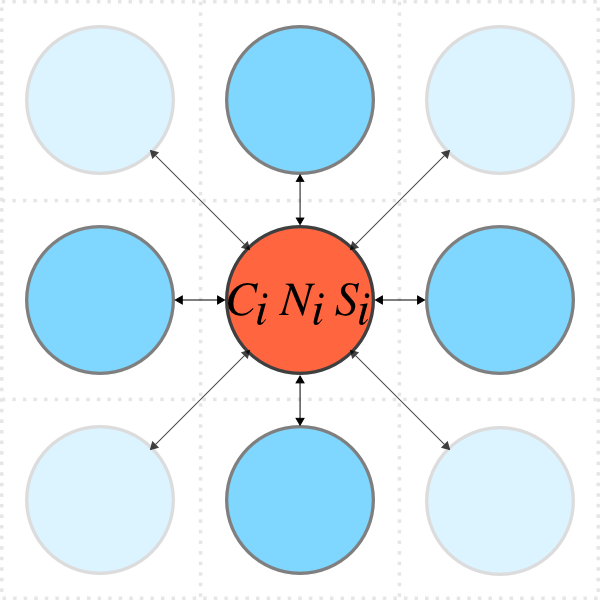
\includegraphics[width=\linewidth]{square_array}
  \captionof{figure}{Schematic of simple modelling approach.}
  \label{fig:simple_model}
\end{Figure}


Models will be written in SBML (ref), using SBML shorthand (ref), so
that they may eventually be published in the BioModels database (ref)
and reused by the scientific community. This will require conformation
to the minimum information standard MIRIAM (ref). (Simulation
experiments should also conform to MIASE (ref).) We will write code
for the rest of the project in Python as this has several advantages:
it is used widely by the scientific community, has libraries which
will be of use to us, and related tools such as Colonyzer (ref) are
already written in Python. To interface SBML models with Python we
will use the libSBMLO library \citep{Bornstein2008}. ODEs will be
solved using odeint from the SciPy library \citep{SciPy}. We will use
git as version control and use GitHub as a remote repository to allow
collaboration and so that tools may eventually be released publicly.

It is anticipated that solving sets of ODEs for typically 384 cultures
in QFA and 1536 cultures in SGA will be take a long time. Therefore,
while testing, we will simulate smaller sets of artificial data from
the ODE models and attempt to fit these. We will also incorporate
unittesting into the development to try to ensure that the code will
still work when scaled up to larger arrays used in experiments.

When dealing with experimental data we must also consider how to treat
cultures around the edge of the agar. These have access to
proportionally more nutrients because there is a large area at the
edge of the plate which is unoccupied. In photographic images, these
sites are also affected by reflections from plate walls which cause
errors in intensity measurements, a proxy for cell density, which
cannot be fully corrected for by Colonyzer \citep{Lawless2010}. In
experiments, an identical culture is grown in these locations and the
results are discarded (see refs). We may choose to adjust for the
increased nutrient availability and include these sites in our model
and analysis. This would introduce a systematic error for sites close
to the plate edges and is an argument for the use of repeats and
randomisation of location (see \ref{sec:comp-exper-designs}). A
simpler modelling approach is to discard the first outer layer
entirely from the model and the second outer layer from the final
results. However, this is undesirable as it reduces the amount of
information that is gathered from each plate and may not account for
the systematic error any better that the more complicated approach,
possibly allowing it to propagate further.

\subsection{Analyse Experimental Data}
\label{sec:analyse-data}
We have access to unpublished QFA and SGA data for the model organism
\textit{S. Cerevisiae}. Some data (Figure~\ref{fig:gaps}), with vacant
gaps, is specifically designed for the study of competition. We will
analyse data from single plates to avoid having to deal with batch
variance which can be a major source of error (see
\citet{Baryshnikova2010}). We will at first fit our model to data
using least squares. The QFA R package (ref) contains functions for
fitting the independent logistic growth model and there is development
underway of a qfaBayes package (ref) which will carry out a Bayesian
inference of parameters of the same model. We plan to develop a method
for Bayesian inference using the CANS model which will account for our
prior knowledge about parameters (?from the independent model?)/the
distributions of parameters (?any other advantages?) (?and allow us to
conduct model comparison?). In an analysis of high-throughput QFA data
from a genetic interaction study by \citet{Addinall2011},
\citet{Heydari2016} use a Bayesian hierarchical model which mirrors
the exerimental structure (from the time-point to population level)
and simultaneously estimates growth parameters and genetic interaction
strength by sharing information between levels. This approach accounts
for differences in replicate fitness variances between different
mutant strains which cannot be efficiently factored into statistical
analyses \citep{Heydari2016}. When looking at the most significant
genetic interactions, for the increased computational time that it
takes (4 weeks vs 3 hours), this analysis does not offer a significant
advantage over an earlier statistical analysis carried out by
\citet{Addinall2011}. However, \citet{Heydari2016} do identify weakly
interacting genes for which there is no previous evidence, and a
hierarchical model which only modelled population dynamics took
significantly less time (1 week). As we are only studying single plates
and not going on to infer genetic interaction strength, there will be
fewer levels in our hierarchy, allowing for a faster computational
time, and the analysis may provide more significant evidence in
identifying competition effects than it does for genetic interactions
(?is this last bit true? ?should we discard this or not?).

\begin{Figure}
  \label{fig:gaps}
  \centering
  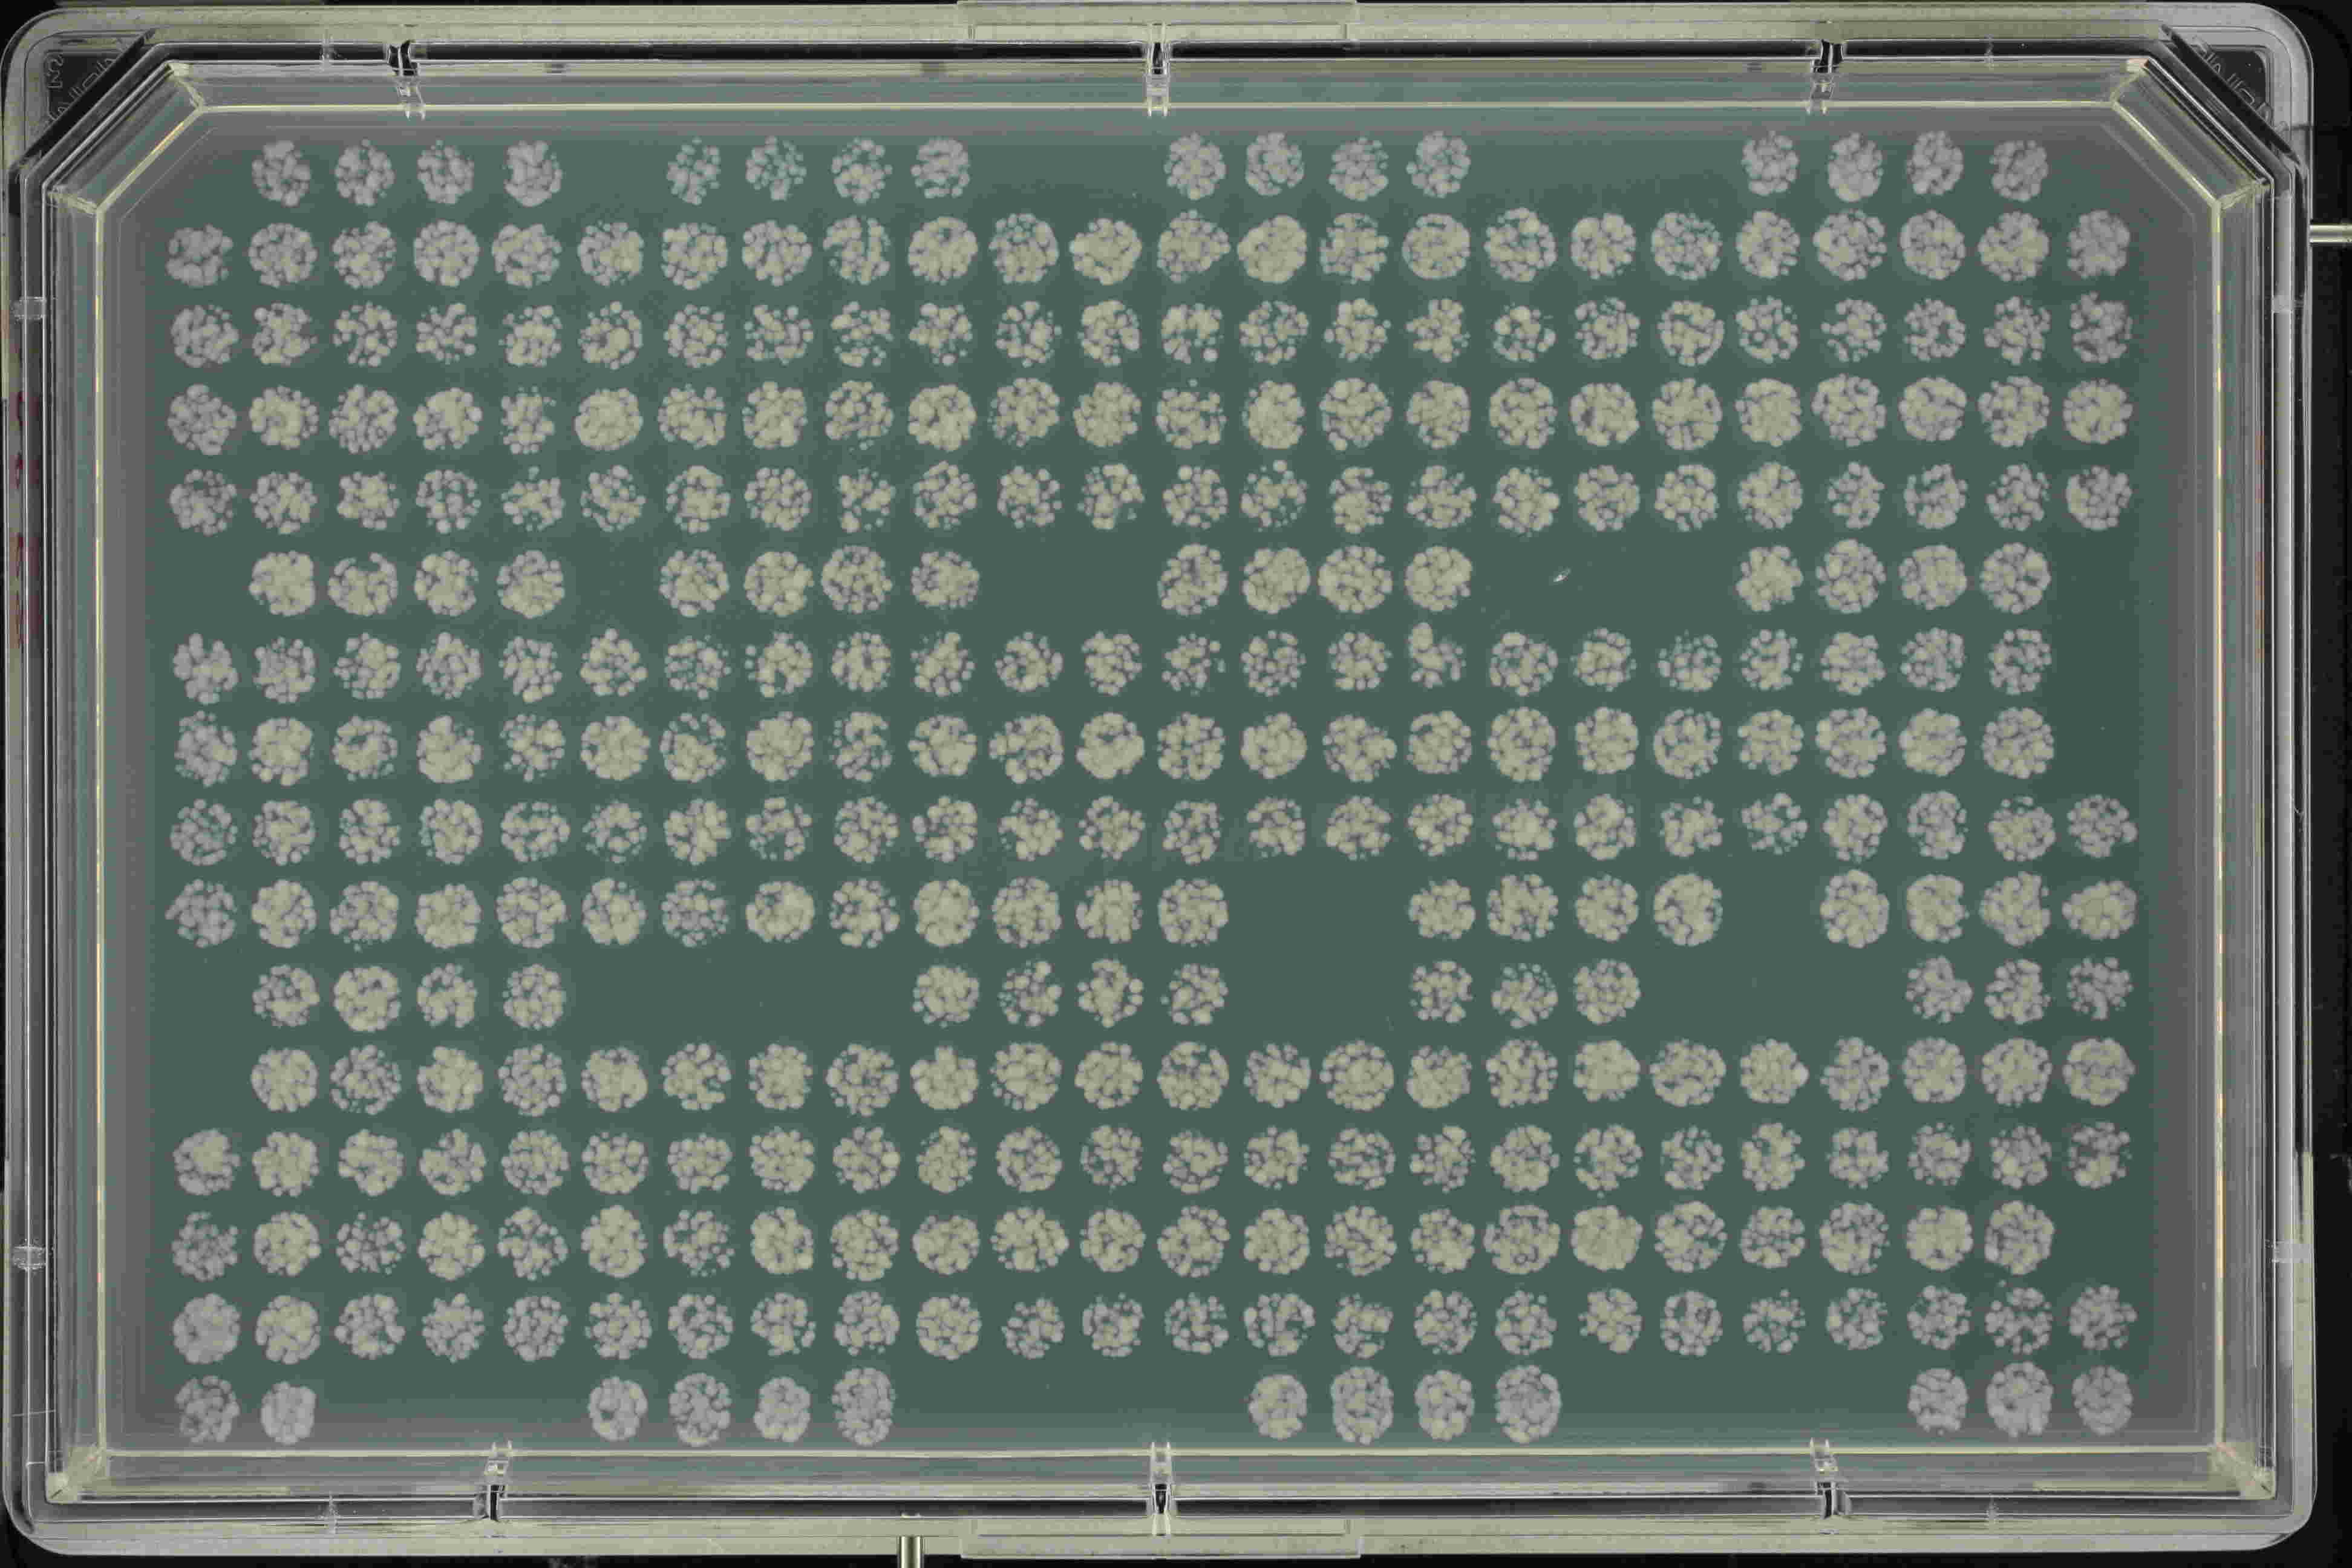
\includegraphics[width=\linewidth]{DLR00012647-2009-07-02_23-12-49}
  \captionof{figure}{An agar with locations left empty (``gaps'')
    designed to exhibit effects of competition and signalling.}
\end{Figure}


If the CANS model is not a good fit to the data, we may need to
improve aspects of our modelling approach (see section
\ref{sec:dev-mod-further}). Otherwise, if competition or signalling
effects provide a significantly better fit to the data, we have proved
our main hypothesis and can move on to comparing experimental designs
(section \ref{sec:comp-exper-designs}. In order to compare diffusion
accross agar height we will also need to develop a two-dimensional
spatially-discretised model of diffusion (section
\ref{sec:dev-mod-further}. We will also determine the effect on
different measures of fitness mentioned in section
\ref{sec:genetic-interaction}(, for both QFA and SGA.)
\subsection{Develop Model Further}
\label{sec:dev-mod-further}

\begin{Figure}
  \centering
  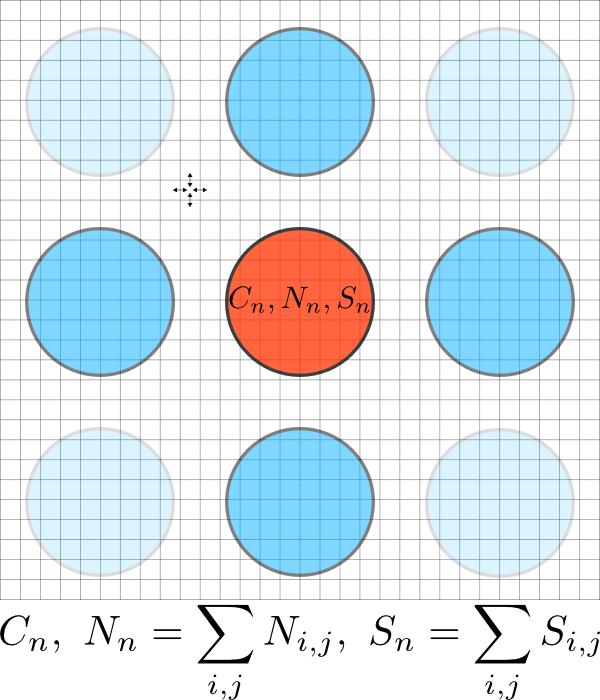
\includegraphics[width=\linewidth]{square_array_grid}
  \captionof{figure}{Schematic of a spatially-discretized two-dimensional model.}
\end{Figure}

\begin{Figure}
  \centering
  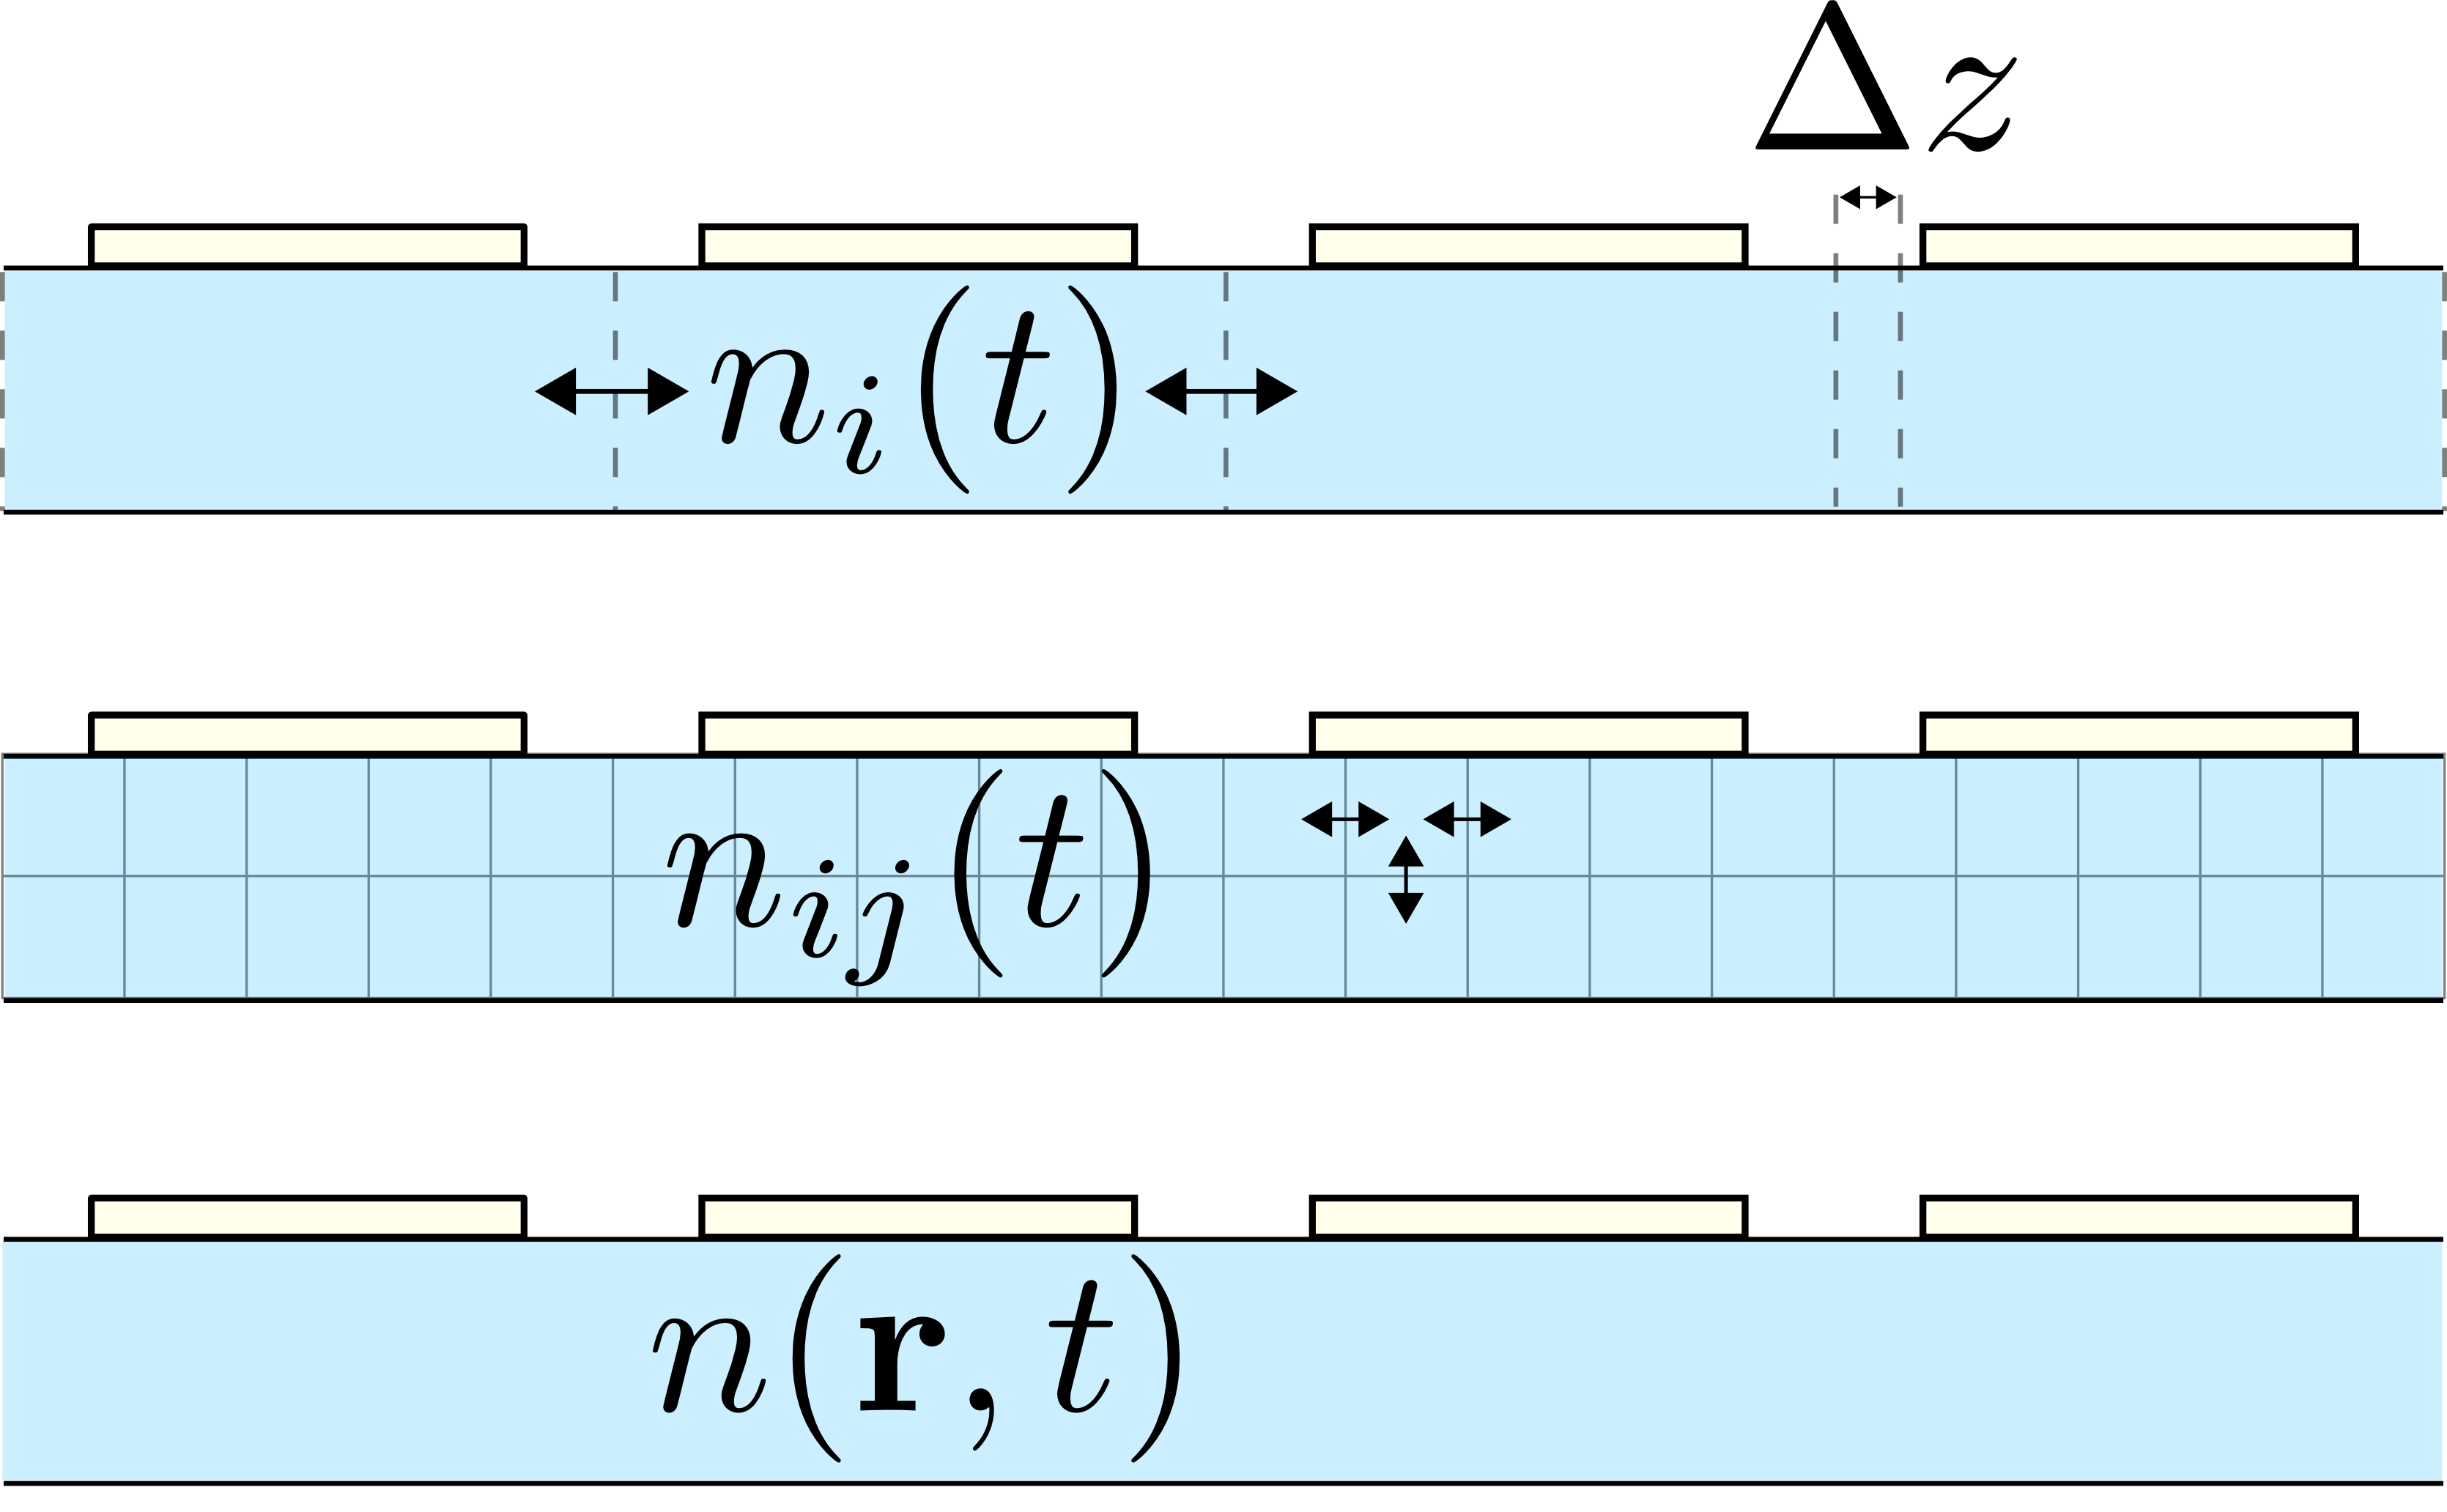
\includegraphics[width=\linewidth]{height_dep_miniqfa_delta_z}
  \captionof{figure}{Schematics of diffusion across agar height.}
\end{Figure}
% Could model movement of vertical or movement across it.
\subsection{Compare Experimental Designs}
\label{sec:comp-exper-designs}


\begin{Figure}
  \centering
  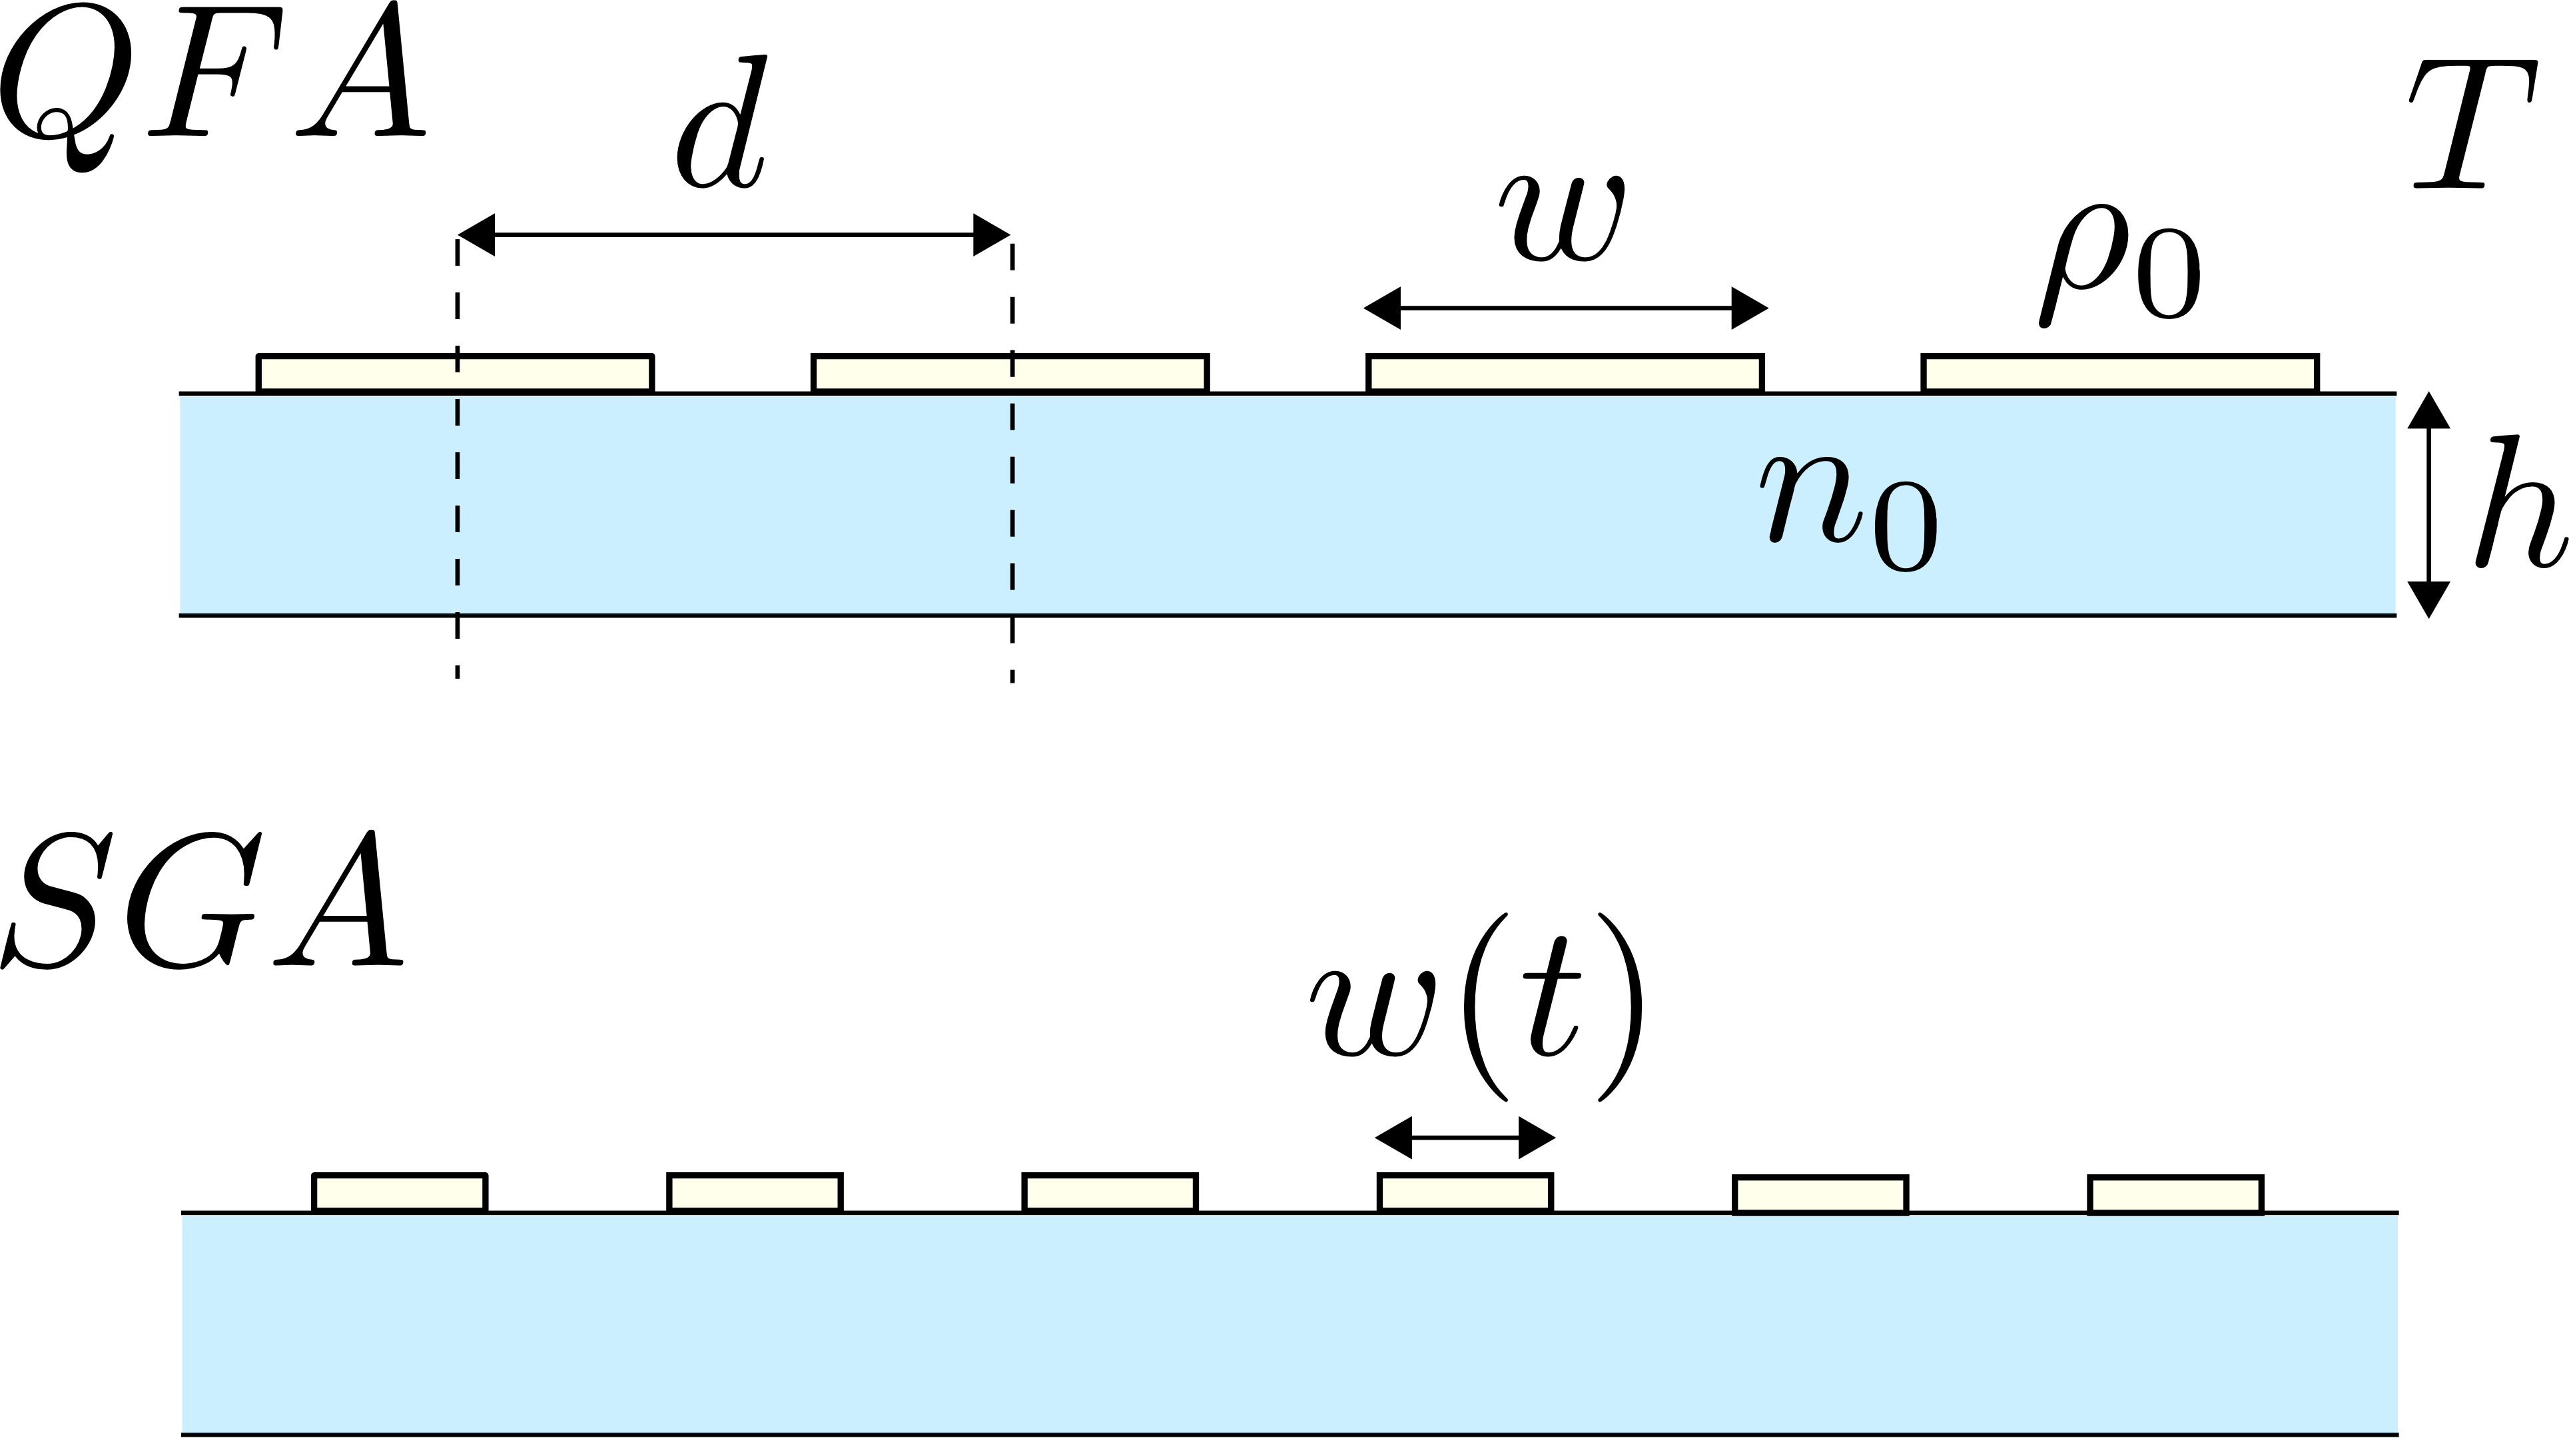
\includegraphics[width=\linewidth]{qfa_v_sga_vars}
  \captionof{figure}{QFA and SGA agars.}
\end{Figure}






\begin{Figure}
  \label{stripes}
  \centering
  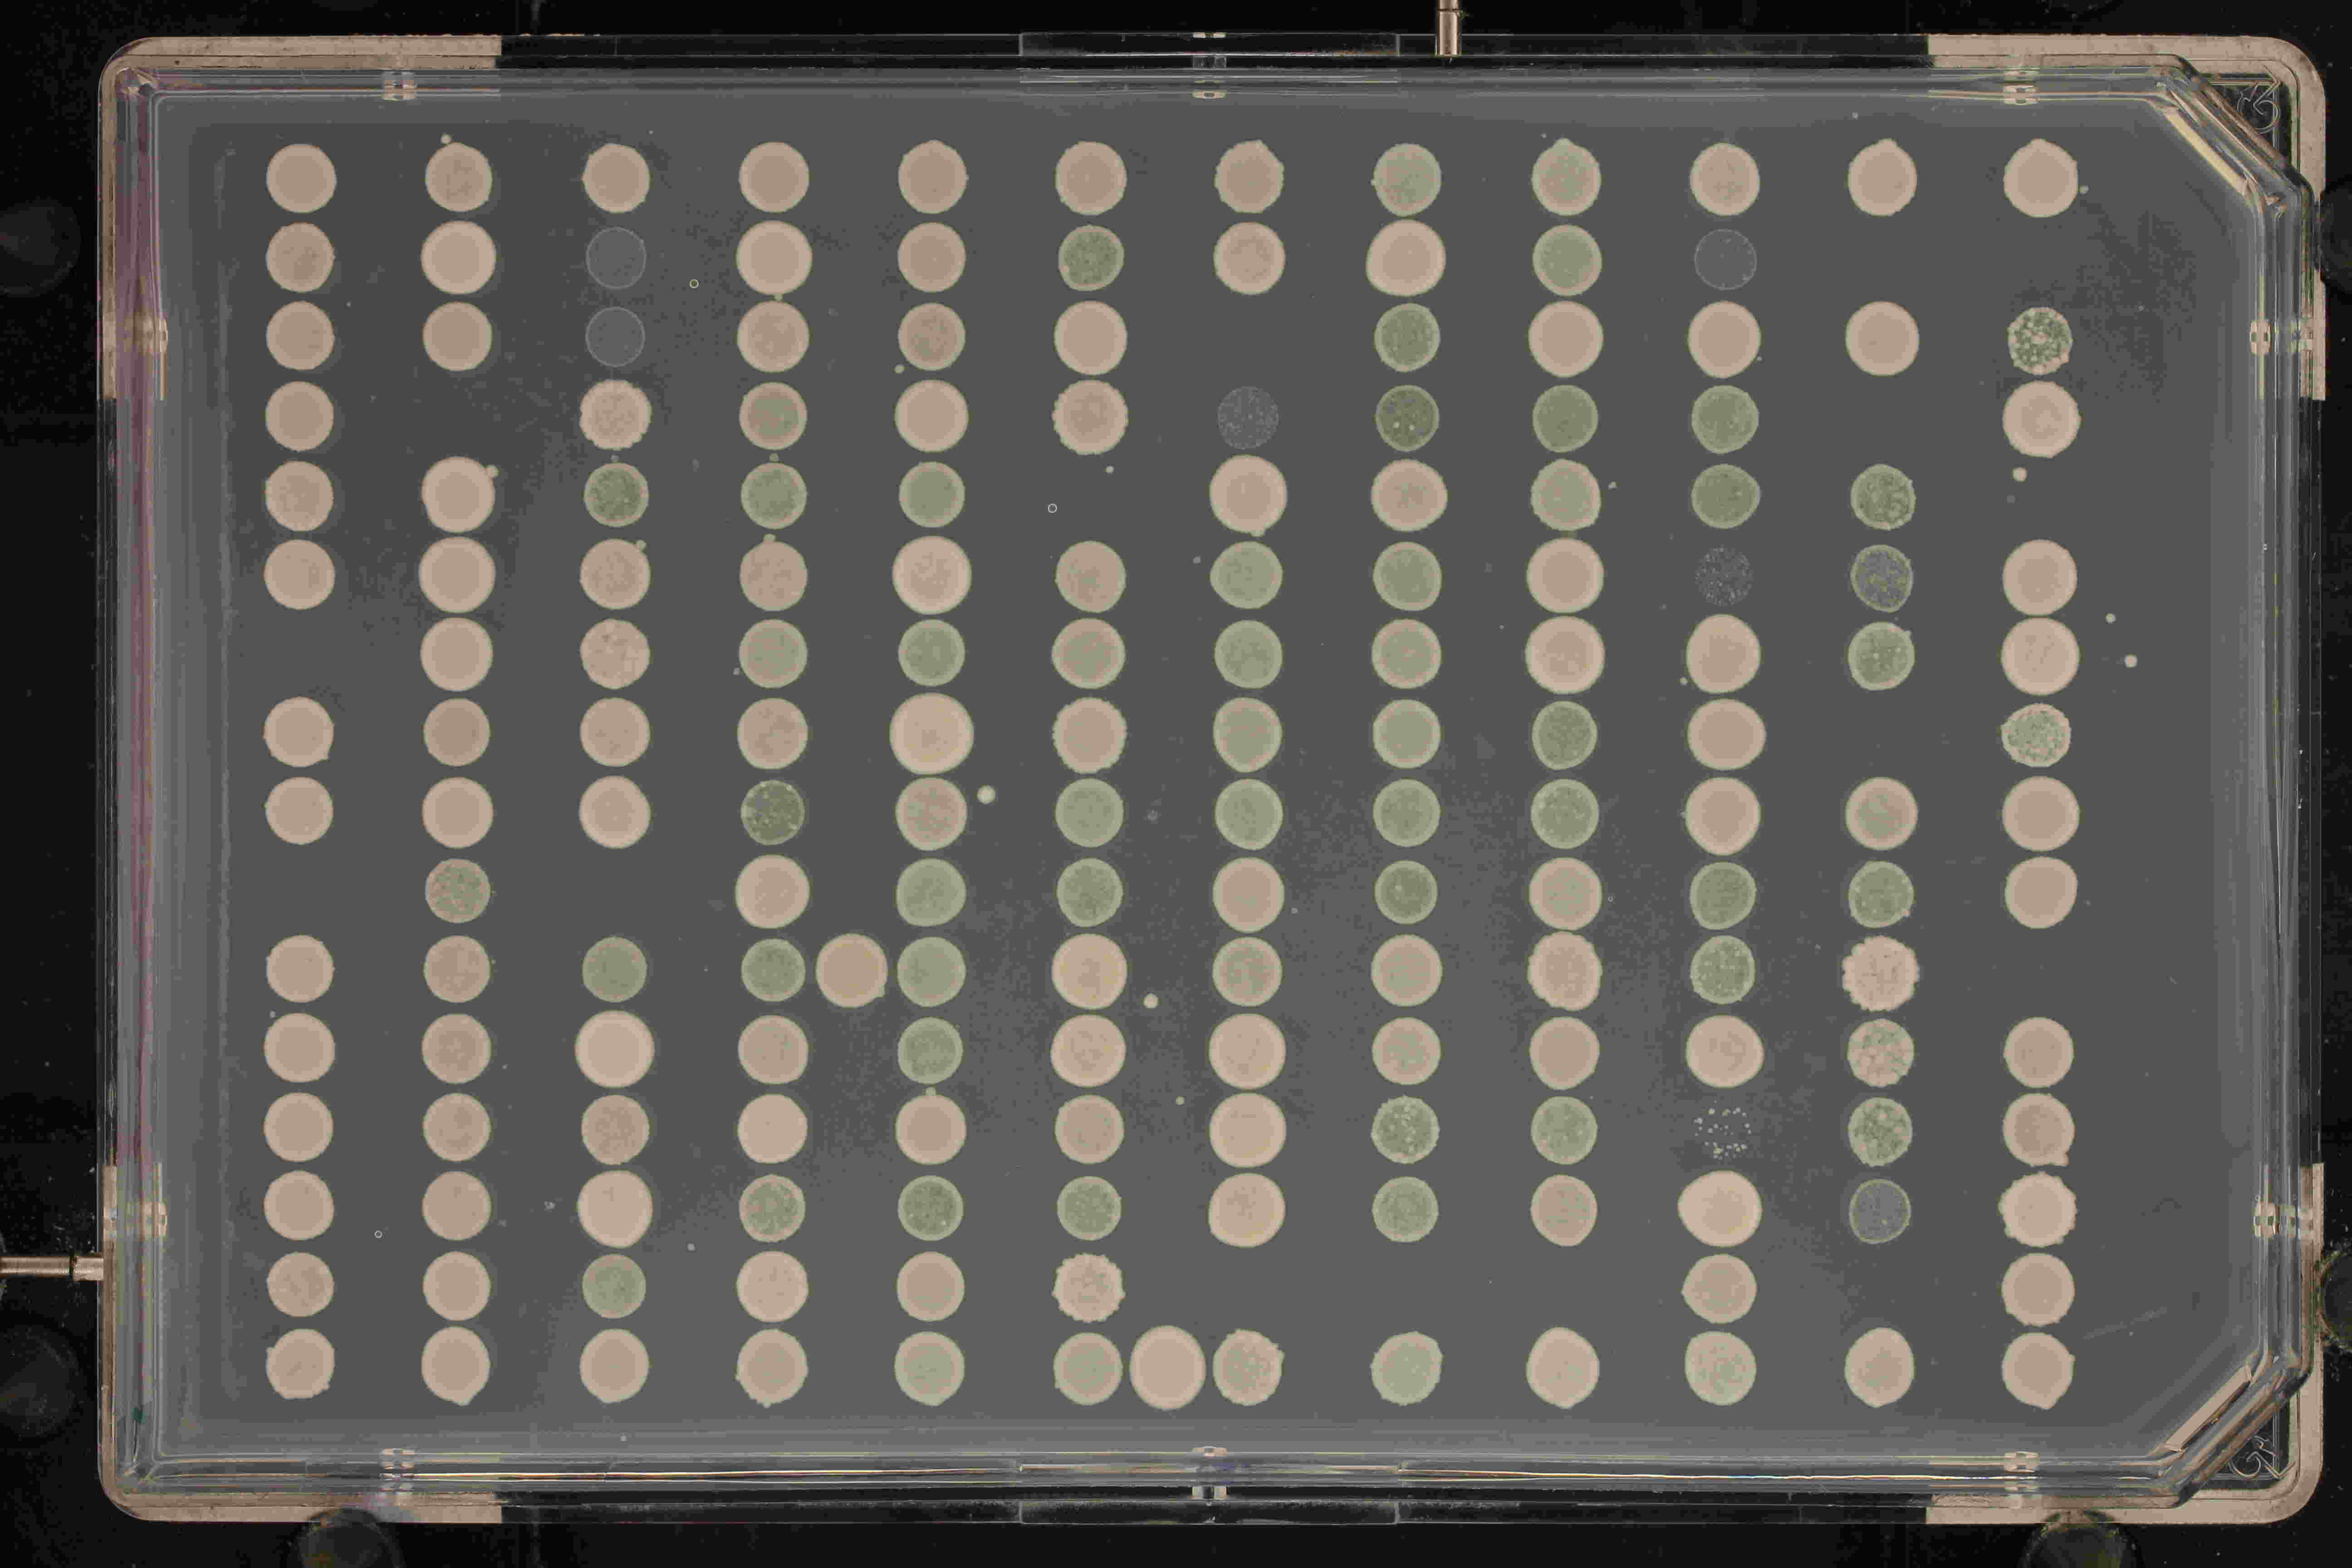
\includegraphics[width=\linewidth]{K000343_027_001_2015-02-21_19-38-08}
  \captionof{figure}{A miniQFA agar in which lines of locations (``stripes'') are left uncultured. We can use a similar experimental setup, with uniform cultures in one dimension, to study diffusion across agar height in only two dimensions.}
\end{Figure}

\subsection{Package and Distribute}
\label{sec:package-distribute}


%%% Local Variables:
%%% mode: latex
%%% TeX-master: "proposal"
%%% End:
